\documentclass[a4paper,12pt]{article}

% Pakiety do różnych funkcji
\usepackage[a4paper,left=2cm,right=2cm,top=\dimexpr15mm+2.5\baselineskip,bottom=3cm]{geometry}
\usepackage{amsmath, amssymb} % For mathematical symbols
\usepackage{multicol}         % Tworzenie wielokolumnowego tekstu
\usepackage{array}            % Ulepszone tabele
\usepackage{graphicx}         % Dodawanie obrazków
\usepackage{float}
\usepackage{color}            % Kolorowanie tekstu
\usepackage{hyperref}         % Hiperłącza w dokumencie
\usepackage{listings}         % Wstawianie kodu źródłowego
\usepackage[utf8]{inputenc}   % Obsługuje kodowanie UTF-8
\usepackage[T1]{fontenc}      % Obsługuje polskie znaki i inne znaki spoza ASCII
\usepackage[polish]{babel}    % Ustawienia języka polskiego
\usepackage{fancyhdr}         % For header and footer
\usepackage{lastpage}         % For total number of pages
\usepackage{lmodern}          % Better font rendering
\usepackage{titlesec}         % For adjusting title spacing
\usepackage{wrapfig}
\usepackage{centernot}
\usepackage{enumitem}
\usepackage[dvipsnames]{xcolor} % Więcej kolorków dla komendy \color
\usepackage{needspace}

% Line spacing adjustments
\linespread{0.8}  % Makes lines less tight
% Header & Footer Setup
\pagestyle{fancy}
\fancyhf{}
\fancyhfoffset[L]{1mm} % left extra length
\fancyhfoffset[R]{1mm} % right extra length
\fancyhead[L]{\textbf{\huge Title}}    % Title on the left (bigger)
\fancyhead[C]{\text{Kacper Poneta \\ Kacper Orszulak \\ Natalia Ignatowicz}} % Author in the middle (bigger)
\fancyhead[R]{\text{\today}}         % Date on the right (bigger)
\fancyfoot[R]{\thepage/\pageref{LastPage}} % Page number in format current/total

% Build info or date on the right of the header
\makeatletter
\@ifundefined{buildHeader}{
  \newcommand{\buildHeader}{\today}
}{}
\makeatother
\fancyhead[R]{\buildHeader}

% Add vertical space before the header line (custom space before the rule)
\renewcommand{\headrulewidth}{0.4pt}    % Header line thickness
\renewcommand{\headrule}{\vspace{10pt}\hrule}  % Add 10pt space above the header line

% Footer setup and add space before the footer line
\renewcommand{\footrulewidth}{0.4pt}    % Footer line thickness
\setlength{\headheight}{50pt}

% Break the page if new section would start near the end of the page
\pretocmd{\section}{%
  \needspace{60ex}%
}{}{}


\fancyhead[L]{\textbf{Projekt sklepu}}    % Title on the left (bigger)

% Document Body
\begin{document}

Lorem ipsum

\begin{figure}[h] % 'h' means here; you can also use 't' for top, 'b' for bottom, etc.
    \centering % Center the figure
    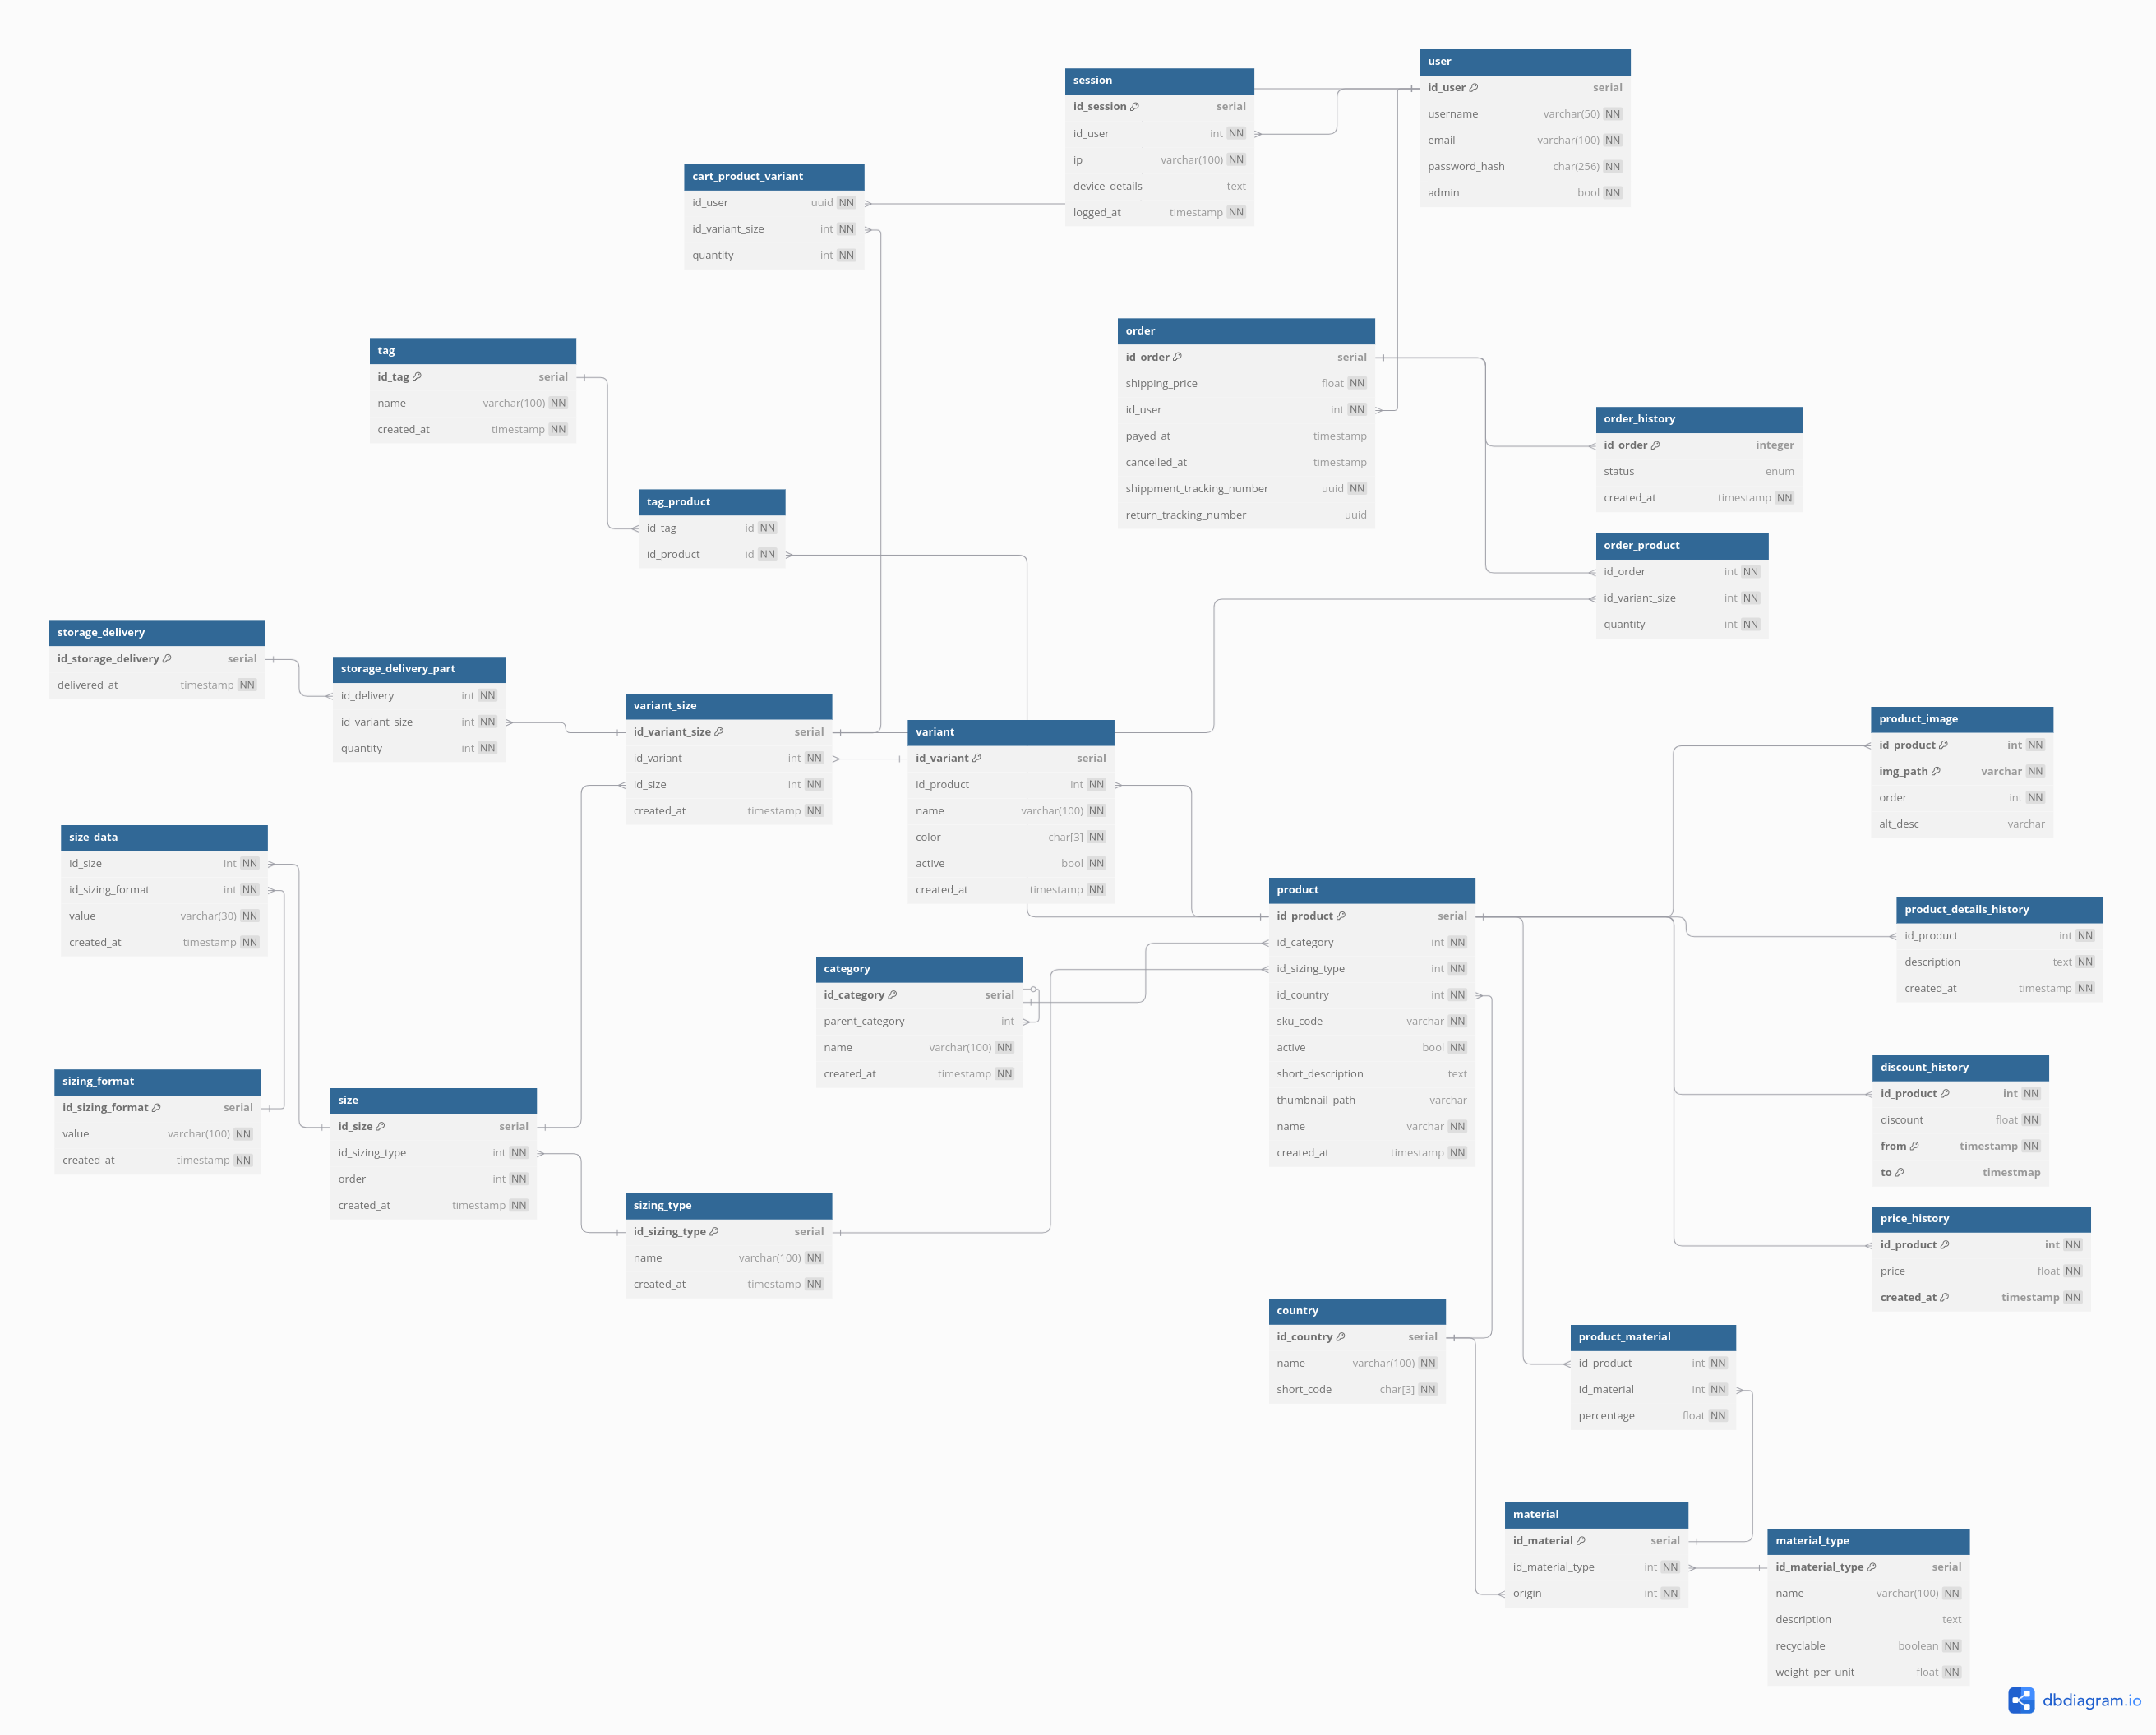
\includegraphics[width=1.0\textwidth]{diagram.png} % Adjust the width as needed
    \caption{This is a caption for the PNG image.} % Optional caption
    \label{fig:example} % Optional label for referencing
\end{figure}

\hfill \break
\section*{Szczegóły niektórych tabel:}

\subsection*{metadata (partial table):}
Wymagane wyzwalacze wymagane przy każdej zmianie tabeli:
\begin{itemize}
    \item {aktualizowanie version}
    \item {aktualizowanie updated\_at}
\end{itemize}

\subsection*{product\_details}
description będzie przechowywany jako markdown. Będziemy go renderować za pomocą biblioteki js.

\subsection*{cart}
Początkowo użytkownik nie będzie posiadał własnego koszyka. Stworzony on będzie, gdy doda coś do niego. UUID koszyka przechowywane będzie w bazie danych PostgreSQLużywając odpowiedniego rozszerzenia. Po stronie użytkownika UUID będzie przechowywane w formie ciasteczka. Koszyk jest aktualizowany za każdym razem, gdy użytkownik wykonuje na nim jakąś akcję. Puste koszyki są od razu usuwane. Dodatkowo każdy koszyk nieużywany odpowiednio długo również jest usuwany za pośrednictwem cronjob.



\end{document}

